\begin{tikzpicture}[node distance=3.4cm and 2.3cm]

    % ----------------------------------------------------------
    % (1) crisp distance matrix  --- interventions × parks
    % ----------------------------------------------------------
    \node[matrixbox] (crisp) {
      \begin{tikzpicture}[scale=0.55,baseline]
        % 5 rows (interventions) × 4 cols (parks)
        \foreach \i in {0,...,5}{
          \draw[very thin,gray!65] (0,\i) -- (4,\i);
        }
        \foreach \j in {0,...,4}{
          \draw[very thin,gray!65] (\j,0) -- (\j,5);
        }
      \end{tikzpicture}
    };
    \node[below=4pt of crisp,align=center]
      {\scriptsize Crisp distance matrix $\mathbf{D}$\\[-1pt]\scriptsize (interventions $\times$ parks)};
    
    % ----------------------------------------------------------
    % (2) stack of 5 membership matrices (5×4 each)
    % ----------------------------------------------------------
    \foreach \name/\x/\col in {close/0/closec,midclose/1/midclosec,mid/2/midc,midfar/3/midfarc,far/4/farc}{
      \node[fuzzymatrix=\col,right=of crisp,xshift={(\x)*0.34cm-0.34cm}] (M\name){
        \begin{tikzpicture}[scale=0.23] % 5×4 tiny grid
          \foreach \i in {0,...,5}{
            \draw[very thin,white] (0,\i) -- (4,\i);
          }
          \foreach \j in {0,...,4}{
            \draw[very thin,white] (\j,0) -- (\j,5);
          }
        \end{tikzpicture}
      };
    }
    \node[below=4pt of Mmid,align=center]
      {\scriptsize 5 fuzzy membership matrices\\[-1pt]\scriptsize (one per linguistic term)};
    
    % ----------------------------------------------------------
    % (3) aggregated membership vector (t-conorm)
    % ----------------------------------------------------------
    \node[matrixbox,right=of Mmidfar,xshift=1.1cm] (agg) {
      \begin{tikzpicture}[scale=0.65,baseline]
        % 5×1 column vector grid
        \foreach \i in {0,...,5}{
          \draw[very thin,gray!65] (0,\i) -- (1,\i);
        }
        \draw[very thin,gray!65] (0,0) -- (0,5);
        \draw[very thin,gray!65] (1,0) -- (1,5);
        % shade only the 1st, 3rd and 5th cells
        \foreach \y in {0,2,4}{
          \fill[closec!28] (0,\y) rectangle ++(1,1);
        }
      \end{tikzpicture}
    };
    \node[below=5pt of agg,align=center]
      {\scriptsize aggregated memberships\\[-1pt]\scriptsize per intervention. In blue,\\
      \scriptsize active interventions};
    
    % ----------------------------------------------------------
    % (4) daily mass series
    % ----------------------------------------------------------
    \node[matrixbox,right=of agg] (mass) {
      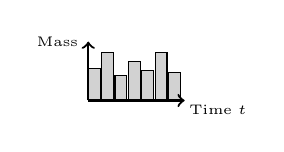
\begin{tikzpicture}[scale=0.34,baseline]
        \foreach \t/\h in {0/1.2,1/1.8,2/0.95,3/1.45,4/1.13,5/1.8,6/1.05}{
          \draw[fill=gray!35] (\t*0.50,0) rectangle ++(0.44,\h);
        }
        \draw[->,thick] (0,0) -- (3.6,0) node[below right=-2pt] {\tiny Time $t$};
        \draw[->,thick] (0,0) -- (0,2.2) node[left] {\tiny Mass};
      \end{tikzpicture}
    };
    \node[below=4pt of mass] {\scriptsize daily mass series $M(t)$};
    
    % ----------------------------------------------------------
    % (5) entropy scores
    % ----------------------------------------------------------
    \node[scalarbox,right=of mass] (entropy)
      {\Large$-\displaystyle\frac{H\!\bigl(M_{\text{norm}}\bigr)}{H_{\text{unif}}}$};
    \node[below=4pt of entropy,align=center]
      {\scriptsize 5 normalised entropy scores\\[-1pt]\scriptsize (one for each fuzzy term)};
    
    % ----------------------------------------------------------
    % arrows
    % ----------------------------------------------------------
    \draw[arrow] (crisp.east) -- ++(1.0,0) -- (Mclose.west)
      node[process,above,yshift=12pt,pos=0]{apply\\linguistic\\ variable};
    
    \draw[arrow] (Mmidfar.east) -- ++(0.9,0) -- (agg.west)
      node[process,above,yshift=12pt,pos=0.4]%
           {row-wise aggregation\\(t-conorm)\par\textbf{for each of the 5}\\membership matrices};
    
    \draw[arrow] (agg.east) -- (mass.west)
      node[process,above,yshift=12pt,pos=0.5]{aggregate\\per day};
    
    \draw[arrow] (mass.east) -- (entropy.west)
      node[process,above,yshift=12pt,pos=0.5]{normalise by\\total mass};
    
    \end{tikzpicture}